%acmart
%IEEEtran
%rbt-mathnotes-formula-sheet
\documentclass{rbt-mathnotes-formula-sheet}
\usepackage[utf8]{inputenc}
\usepackage[pdf]{graphviz}
\usepackage{derivative}
\title{Deep learning notes}

\begin{document}

\section{Observations}
\begin{eqnarray}
    i,j,k,l,L,m,M,n,N,o \in & \mathcal{N} \\
    X \in & \mathcal{R}^{n \times o} \\
    Y \in & \mathcal{R}^{n \times m}
\end{eqnarray}

\section{Neural Network}

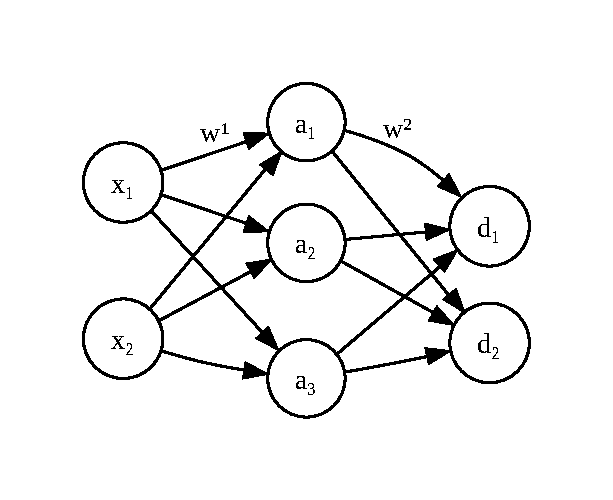
\includegraphics[width=0.3\textwidth]{net.pdf}

\begin{eqnarray}
    a^0 = & x_{1 \times p}(n) \\
    a^L = & d_{1 \times m}(n) \\
    a^l = & \varphi (z^l) \\
    z^l = &  a^{l - 1} W^l
\end{eqnarray}

\section{Gradient Descent}

\begin{eqnarray}
    e(n) = & y(n) - d(n) \\
    \xi(n) = & \frac{1}{2} e e^{\top}\\
    \xi(n) = & \frac{1}{2} \sum_{j=1}^{M} (e_j(n))^2 \\
    W_{(k + 1)} = & W_{(k)} - \nabla_{W} \xi(d,y) \\
    \xi_{avg}(n) = & \frac{1}{2n} \sum_{n=1}^N \sum_{j=1}^{M} (e_j(n))^2 \\
\end{eqnarray}

\section{Backpropagation}

\begin{eqnarray}
    \pdv{\xi}{\omega^l_{ij}} = & \delta_j^l \pdv{z_j^l}{\omega_{ij}} \\
    \delta_j^l = & \pdv{\xi}{z_j^l} \\ 
    \pdv{z_j^l}{\omega_{ij}} = & a_i^{l-1} \\ 
\end{eqnarray}

Output Layer

\begin{eqnarray}
    \delta_j^L =& \pdv{\xi}{z_j^L} = \pdv{\xi}{a_j^L} \pdv{a_j^L}{z_j^L}\\
    \delta_j^L =& \pdv{\xi}{a_j^L} \dot{\varphi}(z_j^L)\\
               =& - e_j \dot{\varphi}(z_j^L)
\end{eqnarray}

Hidden Layer

\begin{eqnarray}
    \delta_j^l = & \pdv{\xi}{z_j^l} = \sum_k \pdv{\xi}{z_k^{l+1}} \pdv{z_k^{l+1}}{z_j^l}\\ 
    \delta_j^l = & \sum_k \delta_k^{l+1} \pdv{z_k^{l+1}}{z_j^l}\\
    \pdv{z_k^{l+1}}{z_j^l} = &
    \frac{\partial}{\partial z_j^l} \left( \sum_j \omega_{jk}^{l+1} \varphi(z_j^l) \right)\\
    \pdv{z_k^{l+1}}{z_j^l} = & \omega_{jk} \dot{\varphi}(z_j^l)\\
    \delta_j^l = & \sum_k \delta_k^{l+1} \omega_{jk}^{l+1} \dot{\varphi}(z_j^l)\\
\end{eqnarray}

\end{document}
